% !TEX encoding = UTF-8 Unicode

\documentclass[a4paper]{article}

\usepackage{color}
\usepackage{url}
\usepackage[T2A]{fontenc} % enable Cyrillic fonts
\usepackage[utf8]{inputenc} % make weird characters work
\usepackage{graphicx}

\usepackage[english,serbian]{babel}
%\usepackage[english,serbianc]{babel} %ukljuciti babel sa ovim opcijama, umesto gornjim, ukoliko se koristi cirilica

\usepackage[unicode]{hyperref}
\hypersetup{colorlinks,citecolor=green,filecolor=green,linkcolor=blue,urlcolor=blue}
\usepackage{amsmath}
%\newtheorem{primer}{Пример}[section] %ćirilični primer
\newtheorem{primer}{Primer}[section]
\newtheorem{definicija}[primer]{Definicija}

\begin{document}

\title{Naslov seminarskog rada\\ \small{Seminarski rad u okviru kursa\\Metodologija stručnog i naučnog rada\\ Matematički fakultet}}

\author{Prvi autor, drugi autor (treći autor)\\ kontakt email prvog, drugog (trećeg) autora}
\date{9.~april 2015.}
\maketitle

\abstract{
	%U ovom tekstu je ukratko prikazana osnovna forma seminarskog rada. Obratite pažnju da je pored ove .pdf datoteke, u prilogu i odgovarajuća .tex datoteka, kao i .bib datoteka korišćena za generisanje literature. Na prvoj strani seminarskog rada su naslov, apstrakt i sadržaj, i to sve mora da stane na prvu stranu! Kako bi Vaš seminarski zadovoljio standarde i očekivanja, koristite uputstva i materijale sa predavanja na temu pisanja seminarskih radova. Ovo je samo šablon koji se odnosi na fizički izgled seminarskog rada (šablon koji \emph{morate} da ispoštujete!) kao i par tehničkih pomoćnih uputstava. Molim Vas da kada budete predavali seminarski rad, imenujete datoteke tako da sadrže temu seminarskog rada, kao i imena i prezimena članova grupe (ili samo temu i prezimena, ukoliko je sa imenima predugačko). Predaja seminarskih radova biće isključivo preko web forme, a NE slanjem mejla.
	Popularnost funkcionalnih programskih jezika je u neprekidnom usponu. Sve više čujemo o njihovoj upotrebi u važnim, čak kritičnim delovima softvera za koje moramo da umemo da garantujemo sigurnost i korektnost izvršavanja. Osim pitanja korektnosti, danas, kada brzina računarskih mašina raste iz dana u dan, postavlja se pitanje efikasnosti implementacije programa napisanih u nekom funkcionalnom programskom jeziku. U ovom radu predstavićemo osnovne tehnike implementacije, ali i sažeti neke koje se koriste u efikasnim kompilatorima za jezike kao što je Haskell. Takođe, prikazaćemo načine dinamičkog upravljanja memorijom kroz koncept sakupljača otpadaka i opisati značajne virtualne mašine za kompiliranje funkcionalnih programskih jezika.
}

\tableofcontents

\newpage

\section{Uvod}
\label{sec:uvod}

% Concepts of programming languages (0th edition).pdf, str. 672
% backus.pdf
Funkcionalna paradigma, koja se zasniva na matematičkim funkcijama, predstavlja osnovu dizajna najznačajnijih stilova jezika koji nisu imperativni. Džon Bakus\footnote{John Backus (1924 -- 2007)} je 1977. godine dobio Tjuringovu nagradu\footnote{ACM Turing Award (\url{http://amturing.acm.org/})} za njegov doprinos u razvoju imperativnog jezika FORTRAN. Prilikom zvaničnog uručenja nagrade 1978. godine, Bakus je održao govor u kojem je izneo argumente zašto su čisti funkcionalni programski jezici bolji od imperativnih programskih jezika. Srž njegovih argumenata je bila da se programi napisani na čisto funkcionalnim programskim jezicima jednostavnije razumeju, što pre razvoja, to i nakon razvoja programa \cite{Can-Programming-Be-Liberated-from-the-von-Neumann-Style?, Concepts-of-Programming-Languages}.

% Concepts of programming languages (0th edition).pdf, str. 673
U svom izlaganju, Bakus je predstavio funkcionalni jezik FP da bi potvrdio svoje tvrdnje. Iako sam jezik nije zaživeo, njegova ideja je doprinela raznim debatama na istu temu. Poslednjih decenija, sa pojavom i razvitkom funkcionalnih jezika poput ML, Haskell, OCaml i F\#, poraslo je interesovanje za funkcionalne programske jezike \cite{Concepts-of-Programming-Languages}.

Prilikom izučavanja nekog programskog jezika, ili bolje rečeno, prilikom izučavanja neke paradigme, postavlja se prirodno pitanje načina prevođenja od izvornog do izvršnog k\^oda. Ovaj proces je poznat kao \textit{kompiliranje} (engl. \textit{compilation}). Kompiliranje funkcionalnih programskih jezika ima posebna svojstva u odnosu na opšti proces kompiliranja zbog specijalnih odluka u dizajnu funkcionalnih programskih jezika. Ideja iza ovog rada jeste upoznavanje čitaoca sa nekim osnovnim tehnikama koje se koriste u procesu kompiliranja funkcionalnih programskih jezika.

Nakon uvoda u rad, u delu \ref{sec:osnovni pojmovi} upoznaćemo čitaoca sa osnovnim pojmovima na koje ćemo se pozivati u daljem tekstu. Prvo, govorićemo o \textit{lambda računu}, formalizmu koji predstavlja osnovu za kompiliranje funkcionalnih programskih jezika. Naravno, odabrani su samo oni pojmovi koji su bitni za izlaganje u radu, a za detaljnije upoznavanje sa lambda računom čitalac može konsultovati \cite{Introduction-to-Combinators-and-Lambda-Calculus}. Nakon toga, čitalac se kratko uvodi u pojam \textit{polimorfizma} i, posebno, \textit{parametarski polimorfizam}.

Deo \ref{sec:efikasan kod} je posvećen tehnikama kojima se dobija efikasan k\^od. U tom delu upoznajemo čitaoca sa \textit{transformacijama lambda računa}. Od svih transformacija, akcenat stavljamo na \textit{umetanje}, a zatim prelazimo na \textit{uparivanje šablona}. Literaturu za ovu oblast predstavlja pre svega \cite{the-implementation-of-functional-programming-languages}, a zatim i \cite{compilation-by-program-transformation, haskell-by-program-transformation, secrets-haskell-compiler-inliner, compiler-design, compiling-fl}.

Deo \ref{sec:provera tipova} uvodi pojam polimorfizma u funkcionalnim programskih jezicima i obrađuje se značaj parametarskog polimorfizma. Na kraju je prikazan osnovni algoritam za \textit{zaključivanje tipova}. Više o ovoj temi se može pronaći u \cite{the-implementation-of-functional-programming-languages, basic-typechecking}.

Zbog svih zahteva koji su postavljeni pred funkcionalnim programskim jezicima dinamičko upravljanje memorijom mora biti obezbeđeno. Zato, u delu \ref{sec:djubretar}, obrađeni su \textit{sakupljači otpadaka}. Dajemo motivaciju za njihovo korišćenje, a zatim i opise mnogobrojnih tipova sakupljača otpadaka koji su se koristili kroz istoriju \cite{appel, mcca60, col60, feni69, app87}. Literaturu za ovu oblast predstavlja pre svega \cite{the-implementation-of-functional-programming-languages}.

U finalnim delovima \ref{sec:secd-masina} i \ref{sec:Gmasine} opisujemo \textit{virtualne mašine za kompiliranje} funkcionalnih programskih jezika. U tekstu ćemo govoriti o \textit{SECD mašini} i \textit{G mašini}. Predstavićemo njihove arhitekture i prikazati nekoliko primera prevođenja.

\section{Osnovni pojmovi}
\label{sec:osnovni pojmovi}

\subsection{Lambda račun}
\label{subsec:lambda racun}

% the impl. of func... strane 9, 10
U ovom delu ćemo se upoznati sa osnovama lambda računa\footnote{Zapravo, govorićemo o \textit{primenjenom lambda računu} (engl. applied lambda calculus) koji zapravo obuhvata \textit{čist lambda račun} (engl. pure lambda calculus) uz predefinisane konstante, odnosno, vrednosti i operacije na koje smo navikli, poput sabiranja dva prirodna broja. Ipak, u tekstu ćemo pisati ‚‚lambda račun'' misleći na ‚‚primenjeni lambda račun''.}, na koji ćemo se oslanjati u daljem tekstu. Lambda račun ima dva važna svojstva zbog kojeg predstavlja spojnicu između funkcionalnih jezika i njihove implementacije, i to su \cite{the-implementation-of-functional-programming-languages}:
\begin{enumerate}
	\item jednostavnost -- lambda račun ima tek nekoliko sintaksičnih konstrukcija ijednostavnu semantiku.
	\item izražajnost -- lambda račun je dovoljno moćan da se pomoću njega mogu izraziti svi funkcionalni programi (važi i više: sve izračunljive funkcije).
\end{enumerate}

Pređimo na sintaksu lambda računa. Ako imamo funkciju \verb|f| i njene parametre \verb|x1, x2, ..., xn|, onda se \textit{primena} (engl. application) funkcije \verb|f| na argumente \verb|a1, a2, ..., an| zapisuje u infiksnom formatu
\begin{center}
	\verb|(f a1 a2 ... an)|
\end{center}
Na primer, sabiranje brojeva $2+3$ se zapisuje \verb|(+ 2 3)|.

Da bismo razumeli kako se funkcionalni program izvršava, prvo ćemo uvesti pojam redukcije. Neformalno, kažemo da se izraz \verb|A| \textit{redukuje} (engl. reduce) na izraz \verb|B| ako su izrazi \verb|A| i \verb|B| ekvivalentni i tada se izraz \verb|A| zamenjuje izrazom \verb|B|. Na primer, izraz \verb|(+ 2 3)| možemo zameniti izrazom \verb|5| (jer je $2+3=5$). Iz samog konteksta čitaocu bi trebalo ovo da bude jasno, te nećemo uvesti formalno pojam redukcije. O formalnom uvođenju redukcije može se pronaći više u \cite{foundations-of-functional-programming}. Redukciju ćemo označavati simbolom $\rightarrow$. U skladu sa prethodnim primerom važi \verb|(+ 2 3)| $\rightarrow$ \verb|5|.

Sa stanovišta implementacije, funkcionalni program treba posmatrati kao \textit{izraz} (engl. expression), koji se izvršava tako što se \textit{izračunava} njegova vrednost (engl. evaluate). Proces izračunavanja se sada vrši biranjem \textit{reducibilnog izraza} (engl. reducible expression) i njegovim redukovanjem \cite{the-implementation-of-functional-programming-languages}. Na primer, neka treba izračunati izraz \verb|(+ (* 5 6) (* 8 3))|. U ovom izrazu postoje dva reducibilna izraza, \verb|(* 5 6)| i \verb|(* 8 3)|. Ceo izraz nije reducibilan izraz jer funkcija \verb|+| mora da se primeni nad dva broja. Proizvoljnim biranjem prvog reducibilnog izraza, pišemo
\begin{center}
	\verb|(+ (* 5 6) (* 8 3))| $\rightarrow$ \verb|(+ 30 (* 8 3))|
\end{center}
Sada je preostao tačno jedan reducibilni izraz, pa pišemo
\begin{center}
	\verb|(+ 30 (* 8 3))| $\rightarrow$ \verb|(+ 30 24)|
\end{center}
Ovom redukcijom je nastao novi reducibilni izraz, pa pišemo
\begin{center}
	\verb|(+ 30 24)| $\rightarrow$ \verb|54|
\end{center}

% the impl. of func... strane 12, 13
Lambda račun ima posebnu konstrukciju koja se naziva \textit{apstrakcija} (engl. abstraction), kojom se uvode nove funkcije. Apstrakcija ima oblik
\begin{center}
	\verb|(|$\lambda$\verb|x.E)|
\end{center} 
gde je $\lambda$ oznaka za apstrakciju, \verb|x| parametar funkcije, \verb|E| izraz, odnosno, telo funkcije i \verb|.| separator parametra i tela funkcije. Na primer, izraz \verb|(|$\lambda$\verb|x.+ x 1)| označava funkciju koja izračunava sledbenika broja \verb|x|.


\section{Efikasan k\^od}
\label{sec:efikasan kod}

% Compilation_of_Functional_Languages_by_Program_Tra.pdf

Jedan od najvažnijih problema vezanih za funkcionalne jezike jeste efikasnost izvršavanja. 
U nastavku opisujemo tehnike koje se koriste za generisanje efikasnog k\^oda.	


\subsection{Transformacije lambda računa}

Već smo napomenuli da se lambda račun koristi zbog svoje jednostavnosti, kao i da je dovoljno izražajan da se bilo koji funkcionalan jezik može transformisati u njega. To znači da ako imamo implementaciju lambda računa, možemo da implementiramo bilo koji funkcionalan jezik tako što ćemo ga prevesti u lambda račun. Transformacije se često grupišu u dva skupa \cite{compilation-by-program-transformation}:

\begin{itemize}
	\item Veliki skup jednostavnih, lokalnih transformacija koje su implementirane u okviru dela kompilatora koji nazivamo \textit{pojednostavljivač} (engl. \textit{simplifier}). Složenost programa raste jer pojednostavljivač pokušava da izvrši što je moguće više transformacija u jednom prolasku kroz program. Uprkos tome, rezultat nakon tih transformacija često i dalje sadrži delove koji mogu biti dalje transformisani, tako da se ova operacija ponavlja više puta, dokle god ima nešto da se pojednostavi. Transformacije koje spadaju u ovaj skup su simplifikacija (engl. \textit{simplification}) \cite{compilation-by-program-transformation}, $\beta$-odsecanje, umetanje (engl. \textit{inlining}) i \textit{sklapanje konstanti} (engl. \textit{constant folding}).
	
	\item Manji skup složenijih, globalnih transformacija, od kojih se svaka implementira odvojeno. Mnoge se sastoje od faze analize praćene transformacijama koje koriste rezultate analize za otkrivanje pogodnih delova za transformisanje. Mnogi se oslanjaju na to da će pojednostavljivač ‚‚počistiti'' k\^ od koji proizvedu, tako da se izbegava ponavljanje transformacija koje su već sadržane u telu pojednostavljivača. Primer transformacije za ovaj skup je  \textit{analiza strogosti} (engl. \textit{strictness analasys}) \cite{haskell-by-program-transformation}. 
\end{itemize}

\subsection{Umetanje}
% inline.pdf str. 2
Umetanje funkcijskih poziva je dobar metod za unapređivanje performansi programa koji se sastoji iz malih funkcija, kao što je čest slučaj sa funkcionalnim jezicima. Osnovni princip umetanja je sledeći: poziv funkcije zamenjuje se njenim telom. Umetanje uklanja neke pozive funkcija, ali jednako je važno da spaja k\^ od koji je prethodno razdvojen i zbog toga se implementira u okviru pojednostavljivača \cite{compilation-by-program-transformation}.

Korisno je definisati tri različite transformacije koje zajedno implementiraju ono što neformalno opisujemo kao ‚‚umetanje'' \cite{secrets-haskell-compiler-inliner, compilation-by-program-transformation}:
\begin{itemize}
	\item \textit{Samo umetanje} (engl. \textit{inlining itself}) zamenjuje sva pojavljivanja vezane promenljive kopijom desne strane njene definicije. Pogledajmo to na primeru.
	\begin{primer} ~
		\begin{center}
			\verb|let {f = |$\lambda$\verb|x.x*4} in (f (a*b - c)) + a*d| \\
			$\stackrel{\text{inline f}}{\longrightarrow}$ \verb|let {f = |$\lambda$\verb|x.x*4} in ((|$\lambda$\verb|x.x*4) (a*b - c)) + a*d|
		\end{center}
	\end{primer}
	
	\item \textit{Eliminacija mrtvog koda} (engl. \textit{dead code elimination}) odbacuje veze koje se više ne koriste. Ovo se najčešće dešava kada je svaka pojava promenljive umetnuta. Nadovežimo se na prethodni primer.
	\begin{primer} ~
		\begin{center}
			\verb|let {f = |$\lambda$\verb|x.x*4} in ((|$\lambda$\verb|x.x*4) (a*b - c)) + a*d| \\
			$\stackrel{\text{dead f}}{\longrightarrow}$ \verb|((|$\lambda$\verb|x.x*4) (a*b - c)) + a*d| 
		\end{center}
	\end{primer}
	
	\item \textit{$\beta$-odsecanje} (engl. \textit{$\beta$-reduction}) jednostavno prezapiše lambda izraz \verb|((|$\lambda$\verb|x.E) A)| u \verb|(let {x = A} in E)|. Nadovežimo se na prethodni primer.
	\begin{primer} ~
		\begin{center}
			\verb|((|$\lambda$\verb|x.x*4) (a*b - c)) + a*d| \\
			$\stackrel{\beta}{\longrightarrow}$ \verb|(let {x = a*b - c} in x*4) + a*d| 
		\end{center}
	\end{primer}
\end{itemize}

\subsection{Uparivanje šablona}

Funkcije nad običnim tipovima, kao i nad strukturiranim algebarskim tipovima \cite{algebraic-types}, mogu se definisati preko različitih \textit{slučajeva} (engl. \textit{case}). Različiti slučajevi dati su \textit{šablonima} (engl. \textit{pattern}), koji se uparuju prema vrednostima tog tipa. Ako šablon odgovara vrednosti, promenljive koje se mogu pojaviti u šablonu su vezane za odgovarajuće promenljive komponente te vrednosti. Pogledajmo kako to radi na jednostavnom primeru. 


\begin{primer}
	Neka imamo šablone \verb|[1; x; y]| $\longrightarrow$ \verb|x*y| i \verb|[z]| $\longrightarrow$ \verb|z|, kao i izraz \verb|[1; 2; 3]|. Vidimo da se dati izraz poklapa sa prvim šablonom. Promenljive \verb|x| i \verb|y| vezuju se za komponente 2 i 3 i vraća se njihov proizvod.
\end{primer}


\begin{primer}
	Računanje $n$-tog fibonačijevog broja u programskom jeziku Haskell dato je k\^odom:
	\begin{verbatim}
	fibonaci n
	|n==0 = 1
	|n==1 = 1
	|otherwise = (fibonaci (n-1))+(fibonaci (n-2))
	\end{verbatim}
	Prilikom evaluacije \verb|(fibonaci x)|, imamo tri slučaja od kojih će jedan biti odgovarajući: prvi je kada je vrednost parametra \verb|x| jednaka \verb|0|, drugi je kada je vrednost parametra \verb|x| jednaka \verb|1|, a treći kada nisu ispunjena prva dva uslova. Uslovi se isprobavaju jedan po jedan, od vrha, dok se ne pronađe odgovarajući šablon \cite{the-implementation-of-functional-programming-languages}.
\end{primer}

Ovakvo poređenje na osnovu šablona naziva se \textit{uparivanje šablona} (engl. \textit{pattern matching}) \cite{compiler-design}.

Uparivanje šablona je zapravo skraćenica za ugnežđene \verb|if-then-else| i \verb|case| naredbe (engl. \textit{statements}): pokušaj da upariš ulaz sa prvim šablonom i ako se poklapa izvrši odgovarajuću akciju, u suprotnom se vrati korak nazad i pokušaj sa sledećim šablonom. Ova strategija proizvodi nepotreban rad. Kompilatori to mnogo bolje rade tako što šablone kompiliraju u \textit{diskriminišuće stablo} (engl. \textit{discrimination tree}) koje to radi u skoro optimalnom broju testova nad podacima kako bi odabralo odgovarajuću akciju \cite{compiling-fl}.


% TODO: pročitajte i dajte svoj sud
% ovo poglavlje je nezvanicno završeno
% potencijalno treba da se dopuni ili lepše zapiše da bi sve delovalo kao jedna celina

\section{Polimorfna provera tipova}
\label{sec:provera tipova}


%The Implementation of Functional Programming Languages strana 139
Neki moderni jezici, kao što je Miranda, imaju svojstvo koje omogućava programeru da ne navodi tipove objekata koje definiše u programu. Kompilator može da odredi tipove ako je to moguće. Deo kompilatora koji se bavi ovim poslom naziva se \textit{zaključivač tipova} \cite{the-implementation-of-functional-programming-languages}. Proveravač tipova je od velike koristi programeru jer mu ukazuje na greške, od trivijalnih propusta u kucanju do velikih logičkih grešaka. Pomaže u pisanju robusnih programa kao i u izgradnji bržih implementacija programskih jezika. Ako zaključivač tipova obradi program, pri izvršavanju se neće javiti greške poput upotrebe promenljive tipa bool kao da je tipa int.
\\
\\ %BasicTypechecking.pdf str. 6
% potrebna referenca za unifikaciju

Izrazi koji sadrže nekoliko pojavljivanja istog tipa, kao $\alpha \longrightarrow \alpha$, izražavaju kontekstnu zavisnost, u ovom slučaju to je zavisnost domena i kodomena tipa funkcije. Proces zaključivanja tipova sastoji se od uparivanja tipova operatora i instanciranja tipova promenljivih. Kad god se tip promenljive instancira, sve ostale pojave iste promenljive moraju biti instancirane sa istom vrednošću: ispravna instanciranja izraza $\alpha \longrightarrow \alpha$ su $int \longrightarrow int$,  $bool \longrightarrow bool$, itd. Proces kontekstnog instanciranja izvodi se pomoću \textit{unifikacije} i ona je osnova polimorfne provere tipova. Unifikacija ne uspeva kada pokušava da upari dva operatora različitih tipova (npr. int i bool) ili kada pokušava da instancira promenljivu izrazom koji sadrži tu promenljivu (npr. $a$ i $a\longrightarrow b$, gde će se napraviti rekurzija bez izlaza) \cite{basic-typechecking}. %The latter situation arises in typechecking self-application (e.g. fun(x) x(x)), which is therefore considered illegal.
U opštem slučaju, tip izraza određuje se pomoću skupa pravila kombinovanja tipova za jezičke konstrukcije i tipova primitivnih operatora. 

\iffalse
%The Implementation of Functional Programming Languages sekcija 8.1
\subsection{Ukratko o notaciji}
%ovo je sve nebitno zapravo, ali neka stoji za sad :D
Tipovi koji su zanimljivi kada je funkcionalno programiranju u pitanju su karakteri, broj, istinitosna vrednost, kao i tipovi torki, lista i funkcija. Kada govorimo o ovim tipovima, koristićemo sledeću notaciju:
$$a::A$$

\noindent što predstavlja promenljivu $a$ koja je tipa $A$. 	
\\
\\ Ako su dati tipovi $A_1, \ldots, A_n$ onda $(A_1, \ldots, A_n)$ predstavlja tip tokre $(a_1, \ldots, a_n)$ za koji važi $a_1::A_1$ i $a_n::A_n$. Bitno je naglasiti da $A_1, \ldots, A_n$ ne predstavljaju iste tipove, odnosno da koordinate jedne torke ne moraju biti sve istog tipa. Takođe, tip torke određuje broj koordinata (odnosno dimenziju torke) i njihove tipove. 
\\
\\ Ako je dat tip $A$ onda je $[B]$ tip liste čiji su elementi tipa $B$. U slučaju da su elementi liste torke, sve torke moraju biti istog tipa. Za razliku od tipa torke, tip liste ne određuje njenu dužinu. 
\\
\\ Ako su dati tipovi $A$ i $B$ koristimo $A \longrightarrow B$ za zapis tipa funkcije $f$ koja se primenjuje na promenljivu $a::A$, a čije vrednosti $(f \quad a)$ su tipa $B$.


\fi 


%BasicTypechecking.pdf str. 9
\subsection{Zaključivanje tipova}
\label{subsec: zakljucivanje tipova}

Osnovni algoritam za zaključivanje tipova opisan je u nastavku \cite{basic-typechecking}.

\begin{enumerate}
	\item Kada se pojavi nova promenljiva $x$, njoj se dodeljuje novi tip promenljive što znači da joj tip mora biti određen u daljem kontekstu u kom se pojavljuje. Par $<x, a>$ se čuva u okruženju koje se pretražuje svaki put kad se pojavi $x$, u kom je $x$ tipa $a$.
	
	\item Kad imamo uslovno grananje, izraz u \textit{if} se uparuje sa bool, dok se \textit{then} i \textit{else} grane ostavljaju nedefinisane kako bi se odredio jedinstven tip za ceo izraz.
	
	\item U apstrakciji $\lambda x.e$, tip za $e$ se zaključuje u kontekstu gde je $x$ povezan sa novim tipom promenljive.
	
	\item U aplikaciji $f(a)$, tip od f se unifikuje sa tipom $A \longrightarrow b$, gde je $A$ tip parametra $a$, dok je $b$ nova tipska promenljiva. Ovo ukazuje na to da $f$ mora biti tipa funkcije čiji domen se unifikuje sa $A$, a $b$ je tip povratne vrednosti.
\end{enumerate}




\section{Sakupljač otpadaka}
\label{sec:djubretar}

%Izvršavanje programa na računaru praćeno je stvaranjem brojnih struktura podataka (objekata).
%Neke od njih generiše sam program, dok su druge vezane za njegovu implementaciju. Sve te strukture podataka se skladište u deo memorije koji se naziva heap.

Strukture podataka koje su alocirane na \textit{hipu} (engl. \textit{heap}), a nisu dostižne preko nekog niza pokazivača programskih promenljivih, nazivaju se \textit{otpaci} (engl. \textit{garbage}). Memorija koju zauzimaju otpaci treba da bude dostupna za alociranje novih struktura podataka. Proces eliminisanja otpadaka, odnosno, njihovog uklanjanja iz memorije naziva se \textbf{sakupljanje otpadaka} (engl. \textit{garbage collection}) i događa se u fazi izvršavanja programa.

\subsection{Motivacija}

Kod proceduralnih programskih jezika, kakav je na primer PASCAL, operacije stvaranja i uništavanja objekata koji se skladište na hipu izvršavaju se eksplicitnim navođenjem određenih naredbi (NEW i DISPOSE) u izvornom k\^odu. To znači da je odgovornost za recikliranje otpadaka na programeru, koji mora da uništi svaki nepotrebni objekat odgovarajućom naredbom i time oslobodi memorijske ćelije zauzete tim objektom. Ukoliko to ne uradi kapacitet memorije se prividno smanjuje. Ova pojava se naziva \textit{curenje memorije} (engl. \textit{memory leak}).

Ovakav koncept je prihvatljiv kod proceduralnih jezika, kod kojih su pomenute operacije retke, ali je neefikasan kada su u pitanju funkcionalni jezici koji se odlikuju čestim izvršavanjem tih operacija \cite{appel}. Zato je kod funkcionalnih programskih jezika posao sakupljanja otpadaka poveren delu sistema za upravljanje memorijom koji se naziva \textit{sakupljač otpadaka} (engl. \textit{garbage collector}).

Različitih tipova sakupljača otpadaka ima mnogo. U daljem tekstu biće predstavljeni neki od njih, kao i njihove osnovne karakteristike.

\subsection{Markirajući sakupljač otpadaka}

Markirajući sakupljač otpadaka je najstariji tip sakupljača otpadaka. Razvijen je početkom 1960-ih godina u okviru programskog jezika LISP \cite{mcca60}.

Programske promenljive i strukture podataka alocirane na hipu formiraju usmeren graf. Promenljive predstavljaju koren tog grafa.

\begin{definicija}
	Kažemo da je čvor \textit{n} \textit{dostižan} u grafu ukoliko postoji put $r\rightarrow \dots \rightarrow n$ od nekog korena \textit{r}.
\end{definicija}

U prvoj fazi, pretragom grafa u širinu se markiraju svi dostižni čvorovi. Ako čvor nije markiran, onda je otpadak i treba da se realocira. Čišćenje hipa se vrši u drugoj fazi počevši od prve adrese i ide do poslednje, pri čemu se traže čvorovi koji nisu markirani. Dobijeni otpaci se povežu u listu koja se naziva \textit{slobodna lista}. Tokom faze čišćenja uklanjaju se markeri svim markiranim čvorovima, da ne bi došlo do problema pri sledećem sakupljanju otpadaka. Nakon što se izvrši sakupljanje otpadaka, prevedeni program nastavlja sa radom.

Kad god program želi da alocira prostor na hipu, on dobija memoriju iz slobodne liste. Kada slobodna lista postane prazna, to je dobar znak da treba opet da se izvrši sakupljanje otpadaka.

\subsection{Sakupljač otpadaka sa brojanjem referenci}
\label{ref:reference counter}

Ideju za ovaj tip sakupljača otpadaka dao je Collins 1960. godine \cite{col60}. On se primenjuje u sistemima kod kojih je hip baziran na listi. Svaka ćelija u hipu sadrži jednu reč koja se naziva \textit{brojač referenci}. Vrednost te reči je broj referenci na ćeliju, tj. broj pokazivača koji na nju pokazuju. Kada se neki podatak smesti u ćeliju i ona postane aktivna, njen brojač referenci dobija vrednost 1. Ako u toku rada program kreira još neki pokazivač na tu ćeliju, njen brojač povećava vrednost za jedan. Ukoliko se uništi neki pokazivač na ćeliju, brojač smanjuje vrednost za jedan. Ako vrednost brojača postane nula, to znači da ne postoji nijedan pokazivač na tu ćeliju, tj. da joj se ne može pristupiti polazeći od nekog korenog pokazivača, pa ona više nije aktivna. Čim ćelija postane neaktivna, reciklira se i to tako što se povezuje u listu slobodnih ćelija.

Ovim se izbegavaju dugotrajni procesi traženja aktivnih ćelija i recikliranja neaktivnih, koji su karakteristični za ostale tipove sakupljača otpadaka. Sve ovo omogućava da se recikliranje otpadaka obavlja paralelno sa izvršavanjem programa, pa je ovaj tip sakupljača pogodan za sisteme u realnom vremenu.

\subsection{Prepisujući sakupljač otpadaka}

Algoritam za ovaj tip sakupljača otpadaka dali su 1969. godine Fenichel i
Yochelson \cite{feni69}. Dostižni deo hipa je usmereni graf, memorijske ćelije su čvorovi, pokazivači su grane, a promenljive su koren.

Prepisujući sakupljač otpadaka prolazi kroz deo grafa koji je alociran na hipu, praveći izomorfnu kopiju u svežem delu hipa. Taj sveži deo je kompaktan i podaci zauzimaju kontinualan blok memorije, bez fragmentacije. Koren sada pokazuje na kopiju, a original se oslobađa. 

Slika \ref{fig:copygc} prikazuje situaciju pre i posle prepisujućeg sakupljanja. Pre sakupljanja, početni prostor je bio pun dostižnih čvorova i otpadaka, nije ostalo mesta za alociranje jer je dostignut limit. Nakon sakupljanja novi prostor između alociranih čvorova i limita je slobodan za alociranje.

\begin{figure}[h]
	\centering
	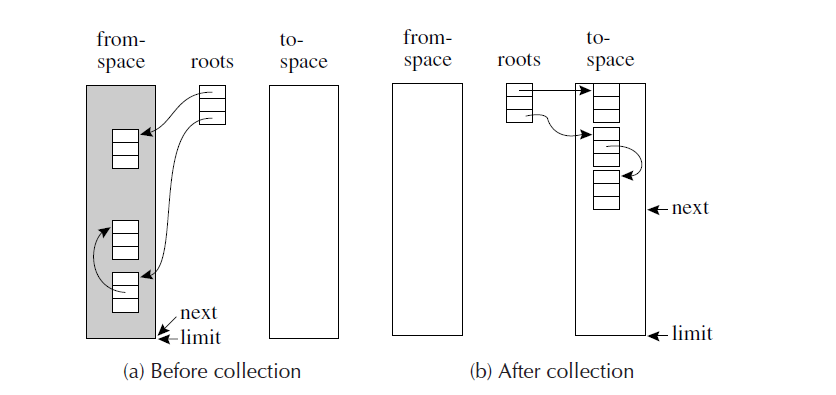
\includegraphics[width=0.9\textwidth]{copygc.png}
	\caption{Prepisujući sakupljač otpadaka.}
	\label{fig:copygc}
\end{figure}

\subsection{Generacijski sakupljač otpadaka}

Jedna od mana prepisujućeg sakupljača otpadaka je što u svakom ciklusu sakupljanja otpadaka premešta sve aktivne ćelije izvornog dela, odnosno, objekte smeštene u njima. To znači da će objekti koji imaju duži životni vek biti premeštani više puta, u toku više ciklusa sažimanja. Ovo ponovljeno premeštanje predstavlja nepotreban posao, koji se može izbeći tako što će se hip podeliti na dva dela.

U jednom delu hipa će se smeštati objekti dužeg životnog veka, što znači da će u njemu biti manje otpadaka, te će proces njihovog sakupljanja moći ređe da se vrši. Drugi će sadržati objekte kraćeg životnog veka i zbog toga će imati veći broj otpadaka, pa će se kompakcija vršiti češće. Strategija koja određuje koliko će se često neki region sažimati naziva se \textit{politika sakupljanja} (engl. \textit{collection policy}).

Postavlja se pitanje kako odrediti koji objekti imaju duži životni vek, tj. kako odrediti koji će se objekti smeštati u koji deo hipa. Empirijske metode su pokazale da većina mladih objekata (onih koji su skoro kreirani) predstavlja privremene strukture ili međurezultate i da samim tim ti objekti imaju kratak životni vek \cite{app87}. Samo mali broj objekata je deo neke strukture dugog životnog veka.

U mnogim stilovima programiranja, kada se kreira objekat A, njegova polja se odmah inicijalizuju i recimo da A pokazuje na objekte B i C. Da bi to bilo moguće objekti B i C moraju već postojati, tako da imamo noviji objekat koji pokazuje na starije objekte. Jedini način da stariji objekat B pokazuje na noviji objekat A je ukoliko je neko polje objekta B izmenjeno dugo nakon kreiranja samog objekta, što je empirijski veoma retko.

\iffalse
\subsection{Odnos prema kompilatoru}

Kompilator za jezik sa sakupljanjem otpadaka uzajamno dejstvuje sa sakupljačem otpadaka generišući k\^od za alociranje podataka, opisujući lokacije za koren svakog ciklusa sakupljanja otpadaka i opisujući izgled podataka na hipu (da li je lista, stek ili stablo). Neki programski jezici i programi, veoma brzo alociraju memoriju na hipu (i generišu otpatke). Ovo je posebno istaknuto kod funkcionalnih programskih jezika, gde je obeshrabreno menjanje starijih podataka.
\fi

\section{SECD mašina}
\label{sec:secd-masina}
%4april
%OVE REFERENCE VEC POSTOJE U TEXTU ALI NE RADE
%@book{landinsecd,
%  title={{The mechanical evaluation of expressions}},
%  author={Peter J. Landin},
%  isbn={9781848822405},
%  url={https://www.cs.cmu.edu/~crary/819-f09/Landin64.pdf},
%  year={1964},
%  publisher={The Computer
%Journal}  
%}

%@misc{ISWIM,
%title = {{The Next 700 Programming Languages}},
%note = {on-line at: \url{http://www.cs.cmu.edu/~crary/819-f09/Landin66.pdf}},
%    author = {Peter J. Landin},
%    year = {1965}
%}
%

Piter Landin napisao je, 1964. godine, članak {\em Mehanička evaluacija} izraza (eng. “The Mechanical Evaluation of Expressions”) \cite{landinsecd}, koji je u decenijama koje predstoje izvršio veliki uticaj na istraživanja i razvoj funkcionalnih programskih jezika. Članak se istakao po tome što je zagovarao upotrebu {\em $\lambda$-računa} kao meta-jezika. Osim toga, Landin uvodi pojmove 'zatvorenja' - da predstavi funkcionalne vrednosti, 'cirkularnost' - da implementira rekurziju, 'parcijalnu evaluaciju', 'redukciju grafa', i mnoge druge koncepte i pojmove koji su danas sastavni deo programskih jezika.\\

Jedna od prvih virtuelnih mašina za kompilaciju funkcionalnih programskih jezika bila je Landin-ova {\em SECD mašina}, predstavljena u članku kao deo ISWIM \cite{ISWIM} programskog jezika. Ona je bila {\em prva apstraktna mašina} posebno dizajnirana da modeluje $\lambda$-račun. \\

Od izlaska Landin-ovog članka, izmišljene, otkrivene i menjane su mnoge druge apstraktne mašine za $\lambda$-račun. Međutim, iako se u literaturi može naći veliki broj mašina, {\em nijedna} nije derivat originalne Landin-ove SECD mašine, čak i pored toga što je ona bila prva.

% O specifičnostima i više informacija može se naći u A Rational Deconstruction of Landin’s SECD Machine Olivier Danvy BRICS ∗ Department of Computer Science University of Aarhus † October 2003

\subsection{Arhitektura SECD mašine}

Osnovna uloga SECD mašine je izvršavanje kompajliranog koda na apstraktnoj mašini. Osnovna razlika u odnosu na interpreter je u tome što kompajlirani kod može da se izvršava više puta i postoji mogućnost optimizacije koda.\\

Formalno, SECD mašina je torka četiri liste koje imaju skup precizno definisanih operacija nad njima. Semantika SECD mašina opisuje virtuelnu mašinu baziranu na steku koja je dizajnirana da izvršava funkcije. \\ 

Komponente torke koje čine SECD mašinu su četiri steka:
\begin{enumerate}
\item {\bf S} (eng. stack) - za evaluaciju izraza, najčešće implementiran kao lista, ova komponenta ima tip {\bf list}  
\item {\bf E} (eng. environment) - za čuvanje liste trenutnih vrednosti u okvirima, gde je svaki okvir lista veza izmedju simbola i njegove vrednosti, ova komponenta ima tip {\bf Env.env}  
\item {\bf C} (eng. control) - za čuvanje liste instrukcija (kontrolnih direktiva) koje treba evaluirati, ova komponenta ima tip {\bf directive} , gde je direktiva definisana kao:\\ datatype directive = TERM of Source.term\\
| APPLY
%ovo iznad treba srediti da se lepo prikazuje
\item {\bf D} (eng. dump) - za čuvanje kontrolnih putanja, promenljivih i stekova, da bi se kasnije mogli ponovo učitati, ova komponenta ima tip\\ {\bf(value list * value Env.env * directive list) list}
\end{enumerate}

%Dump used to store suspended invocation context.
Sada ćemo, u tabeli \ref{tab:tabelaInstr}, predstaviti glavne operacije koje podržava SECD mašina. \\

\begin{table}[h!]
\begin{center}
\caption{Operacije koje podržava SECD mašina}
\begin{tabular}{|c|c|c|c|} \hline
Operacija&Naziv&Opis& Uloga\\ \hline
NIL & & Stavlja NIL pokazivač&\\ \hline
LD & LOAD & Učitava iz E & Dobija vrednost iz konteksta\\ \hline
LDC & LOAD CONSTANT & Učitava konstante&\\ \hline
LDF & LOAD FUNCTION & Učitava funkciju & Dobijanje zatvorenja\\ \hline
AP & APPLY FUNCTION & Primenjuje funkciju&\\ \hline
RTN & RETURN & & \\ \hline
SEL & SELECT & Vrši select ako je u if izrazu&\\ \hline
JOIN & JOIN & Ponovo pridružuje g& Koristi se u kombinaciji sa SEL\\ \hline
RAP & RECURSIVE APPLY & Rekurzivna primena funkcije&\\ \hline
DUM & DUMMY & Kreira 'dummy' env & Koristi se sa RAP\\ \hline
\end{tabular}
\label{tab:tabelaInstr}
\end{center}
\end{table}
%izvor za tabelu je Malkov http://poincare.matf.bg.ac.rs/~smalkov/files/fp.r344.2016/public/predavanja/FP.cas.2016.08.SECD.pdf
%Introduction to Functional Programming Systems Using HaskellАутор: Antony J. T. Davie
Osim operacija navedenih u tabeli imamo {\em ugrađene funkcije} +,
*, ATOM, CAR, CONS, EQ, itd.\\
Svaka operacija je definisana efektom koji ima na četiri steka S,E,C i D. Svaki stek je predstavljen {\em s-izrazom} sa tačka notacijom, gde najlevlja pozicija označava vrh steka.\\

\subsubsection{Ubacivanje objekata na stek}

Pravila kompilacije:
\begin{enumerate}
\item nil se prevodi u (NIL);
\item brojevi ili konstante, koje ćemo označiti sa x, se prevode u (LDC x);
\item identifikator se prevodi u (LD (i,j)) gde je (i.j) indeks u steku E
\end{enumerate}

\begin{primer}
\begin{itemize}
\item NIL S E (NIL.C) D $\rightarrow$ (NIL.S) E C D\\
\item LDC S E (LDC x.C) D $\rightarrow$ (x.S) E C D\\
\item LD S E (LD (i,j).C) D $\rightarrow$ (locate((i,j), e).S) E C D\\
\end{itemize}
\end{primer}
'Locate' je pomoćna funkcija koja vraća j-ti element i-te podliste u E. Primetimo da je E lista podlisti od kojih je svaka lista stvarnih parametara. Iz čega zaključujemo da e odgovara listi vrednosti u interpreteru.

\subsubsection{Ugrađene funkcije}
Pravilo kompilacije: Ugrađena funkcija oblika (OP e1 ... ek) prevodi se u ek' || ... || e1' || (OP), gde A||B označava append(A,B), a ei' je preveden kod za ei. Notacija zamene argumenata i operatora je standardno obrnuta Poljska notacija (postfiksna notacija).
%treba navesti da je svejedno da li su mali secd ili S E C D
Za unarni operator OP,\\
(a.s) e (OP.c) d $\rightarrow$ ((OP a).s) e c d\\
Za binarni operator OP,\\
(a b.s) e (OP.c) d $\rightarrow$ ((a OP b).s) e c d
\begin{primer}
s e (LDC 3 LDC 2 LDC 6 + *.c) d\\
-> (3.s) e (LDC 2 LDC 6 + *.c) d\\
-> (2 3.s) e (LDC 6 + *.c) d\\
-> (6 2 3.s) e (+ *.c) d\\
-> (8 3.s) e (*.c) d\\
-> (24.s) e c d\\
\end{primer}
\subsubsection{Specijalna funkcija IF THEN ELSE}
Pravilo kompilacije:\\
(if e1 e2 e3) se prevodi u {\em e1' || (SEL) || (e2' || (JOIN)) || (e3' || (JOIN))}\\
\begin{primer}
(if (atom 5) 9 7) se prevodi u (LDC 5 ATOM SEL (LDC 9 JOIN) (LDC 7 JOIN))\\
\end{primer}
Operacije na steku:\\
SEL (x.s) e (SEL ct cf.c) d $\rightarrow$ s e c' (c.d)\\
where c' = ct if x is T, and cf if x is F\\
JOIN s e (JOIN.c) (cr.d) $\rightarrow$ s e cr d\\

%Reinhard Wilhelm · Helmut Seidl Compiler Design Virtual Machines ISBN 978-3-642-14908-5 Springer Heidelberg Dordrecht London New York Springer-Verlag Berlin Heidelberg 2010

%G.D. Plotkin, Call-by-name, Call-by-value and the Lambda calculus, 1 August 1974., Department of Machine Imlligence,School of Artificial Intelligence,Edinburgh, United Kingdom

\section{G-mašina}
\label{sec:Gmasine}

U ovom delu predstavićemo {\em G mašinu} (engl. G-machine), koju su Avgustson i Džonson (engl. Augustsson and Johnsson) predstavili u svojim naučnim radovima, na Tehnološkom institutu Čalmers (engl. Chalmers Institute of Technology) u Geteburgu, između 1984. i 1987. godine. 

\subsection{Motivacija}
K\^ od {\em lenjih funkcionalnih jezika}, funkcije i argumenti konstruktora se evaluiraju samo po potrebi, pa čak i onda najviše samo jednom. Bez obzira na to što se ovako nešto može implementirati predstavljanjem neevaluiranih argumenata ‚‚tankovima'' (engl. thunk) - funkcijom koja evaluira argument i zamenjuje ga rezultatom, zbog efikasnosti biramo drugačije pristupe. \\ 
\\Osnovna ideja je da predstavimo program {\em grafom} koji bismo kasnije ‚‚prepisali''  evaluacijom. Velika prednost je i u tome što evaluacija deljenog podgrafa automatski razrešava sve izraze koji pokazuju na njega. Međutim, treba biti pažljiv, kontinuirana pretraga grafa za podizrazima je {\em spora}. \\
\\
Rane implementacije su prevodile program u fiksirani skup kombinatora (zatvorene lambda izraze čije su apstrakcije na početku), koje možemo posmatrati kao pravila za ‚‚prepisivanje grafa''. Kasnije se pokazalo da je korisno prepustiti programu da razmatra izbor kombinatora - tzv. {\em superkombinatora} \cite{super-combinators}. \\ %ovde ide ova ref ] R.J.M. Hughes, Super-combinators: A new implementation method for applicative languages, ACM Symposium on Lisp and Functional Programming, Pittsburgh, Pennsylvania,ACM, August 1982, pp. 1–10.1


\subsection{Osnovna ideja} 
Umesto da interpretiraju superkombinatore kao pravila za prepisivanje grafa, oni se kompajliraju u k\^ od sa specijalnim instrukcijama za manipulaciju grafom. G-mašine su osnova implementacije lenjog ML (engl. lazy ML) \cite{lazy-ML} i Haskela \cite{hbc}.\\ 
%uz Lazy ML ide L. Augustsson, The interactive lazy ML system, J. Funct.Programming 3 (1) (1993) 77–92, A UZ HASKEL ] L. Augustsson, HBC – The Chalmers Haskell compiler,Web Page, 1999, URL: http://www.cs.chalmers.se/augustss/hbc.html.

Osnovna ideja koja stoji iza G-mašina je da se pre pokretanja programa svako telo superkombinatora prevede u niz instrukcija koje, nakon što se izvrše, kreiraju instancu tela superkombinatora. Svaki put samo instanciramo superkombinator, da bismo mogli da odbacimo originalne superkombinatore nakon što je prevođenje završeno, i sačuvamo samo preveden k\^ od. Dakle, koristimo kompajler G-mašine da izvorni k\^ od prevedemo u niz instrukcija na mašinskom jeziku. \\

Nakon što smo preveli telo superkombinatora u niz instrukcija, moramo da odlučimo u koji jezik ćemo da ga prevedemo. Iako bismo mogli odmah da ga prevedemo u, na primer, {\em VAX mašinski k\^ od}, kasnije bi nam se javili mnogi problemi.
Najbolje rešenje, ujedno i ono koje se najčešće koristi, je da prevođenje izvršimo u među k\^ od (engl. intermediate code) za G-mašinu, takozvani {\em G-k\^ od} (engl. G-code). \\

\subsection{G-k\^ od}

{\em G-k\^ od} je k\^ od u koji kompiliramo tela superkombinatora. Kompilator za G-mašinu prati sledeći niz postupaka \cite{the-implementation-of-functional-programming-languages, abstract-machines}:
\begin{enumerate}
\item Izvorni jezik je varijanta ML-a, sa semantikom lenje evaluacije, tzv. {\em lenji ML}.
\item Rane faze kompilacije vrše proveru tipova, nalaženje uzoraka i analizu zavisnosti. U ovoj fazi program je preveden na $\lambda$-račun.
\item $\lambda$-lifter (engl. $\lambda$-lifter) transformiše program u oblik superkombinatora.   
\item Superkombinatori se prevode u G-k\^ od.
\item Konačno, generiše se mašinski k\^ od iz G-k\^ oda za ciljnu mašinu.
\end{enumerate}
%referenca za G kompajler Peyton Jones, Simon L., 1958-The implementation of functional programming languages.'7th May 1986.'Bibliography: p.Includes index.I. Functional programming languages. I. Title.QA76.7.P495 1987 005.13'3 86-20535 ISBN 0-13-453333-X

\iffalse
\begin{figure}[h!]
\begin{center}
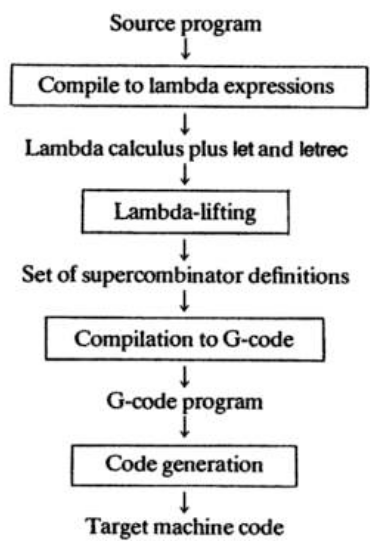
\includegraphics[scale=0.3]{gkomp.png}
\end{center}
\caption{Struktura G-kompajlera}
\label{fig:gcompiler}
\end{figure}
\fi 

\begin{primer}
	Predstavimo sad način na koji funkcioniše kompajler za G mašinu razmatrajući sledeću funkciju:
	$$\text{f g x = K (g x)}$$
	Ova funkcija bi se prevela u sledeći niz instrukcija G-k\^ oda:
	\begin{itemize}
	\item Push 1
	\item Push 1
	\item Mkap
	\item Pushglobal K
	\item Mkap
	\item Slide 3
	\item Unwind
	\end{itemize}
\end{primer}
%referenca za primer i vise info o G masinama Implementing Functional Languages:a tutorial Simon L Peyton Jones Department of Computing Science, University of Glasgow and David R LesterDepartment of Computer Science, University of Manchesterc 1991

\begin{figure}[h!]
	\centering
	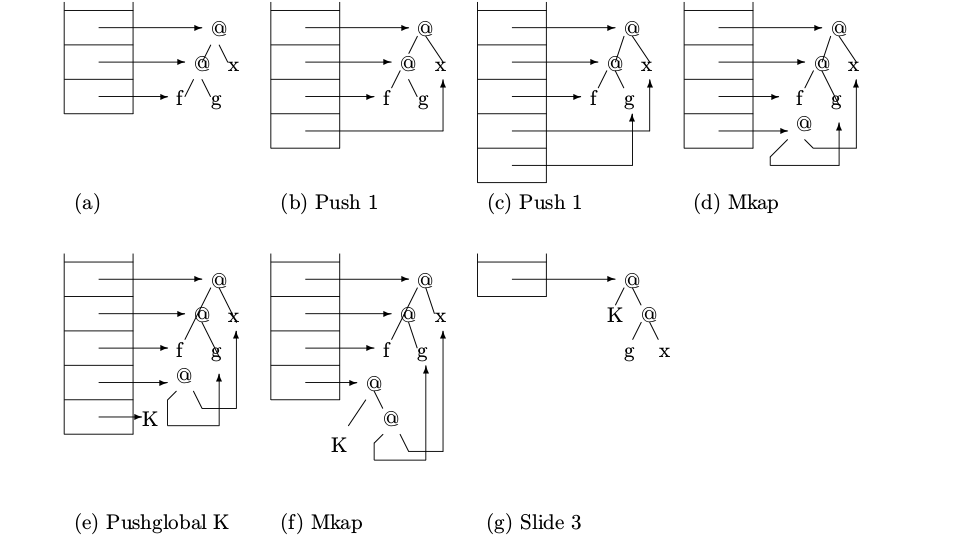
\includegraphics[scale=0.35]{primerGmasine.png}
	
	\caption{Vizuelni prikaz izvršavanja k\^ oda.}
	\label{fig:primerGmasine}
\end{figure}

Na slici \ref{fig:primerGmasine} prikazujemo kako se k\^ od izvršava. Sa leve strane svakog dijagrama prikazan je stek, koji raste nadole. Ostatak svakog dijagrama je hip. Aplikativni čvorovi predstavljeni su karakterom @, izrazi malim slovima, a superkombinatori velikim slovima latinice. Takođe, prikazano je stanje mašine pre izvođenja instrukcija za f. Dva elementa na vrhu steka su pokazivači na aplikativne čvorove, čije su desne strane izrazi koji će biti vezani za g i x. Instrukcija Push koristi relativno adresiranje u odnosu na vrh steka. Ignorišući pokazivač na supekombinatorski čvor f, prvi element na steku dobija broj 0, naredni 1, itd.

Naredni dijagram (b) pokazuje kako se stek izmenio nakon primene Push1 instrukcije. Ona stavlja pokazivač na izraz x na stek. Nakon jos jednog izvršavanja Push1 instrukcije, imamo pokazivač na g na vrhu steka i onda imamo ono što je prikazano na dijagramu (c). Dijagram (d) pokazuje šta se dešava kada se izvrši Mkap instrukcija. Ona uzima dva pokazivača sa steka i pravi aplikativni čvor, ostavljajući pokazivač na rezultat na steku. Na dijagramu (e) izvršavamo Pushglobal K instukciju koja stavlja pokazivač na K superkombinator. Na dijagramu (f) vidimo da još jedna Mkap instrukcija završava instanciranje tela f.\\ 
\\
Sada možemo zameniti originalni izraz f g x  sa novoinstanciranim telom: K(g x). U prvoj (ne lenjoj) verziji G-mašine, jednostavno pomerimo telo nadole za 3 mesta na steku pomoću instrukcije Slide 3 (dijagram (g)).\\ Konačno, Unwind instrukcija uzrokuje dalju evaluaciju.

%za sve ref dodati Abstract machines for programming language implementation Stephan Diehl a,∗, Pieter Hartel b, Peter Sestoft c a FB-14 Informatik, Universität des Saarlandes, Postfach 15 11 50, 66041 Saarbrücken, Germany b Department of Electronics and Computer Science, University of Southampton, Highfield, Southampton SO17 1BJ, UK c Department of Mathematics and Physics, Royal Veterinary and Agricultural University, Thorvaldsensvej 40,DK-1871 Frederiksberg C, Denmark Accepted 24 June 1999



\section{Zaključak}
\label{sec:zakljucak}

Ovde pišem zaključak. 
Ovde pišem zaključak. 
Ovde pišem zaključak. 
Ovde pišem zaključak. 
Ovde pišem zaključak. 
Ovde pišem zaključak. 
Ovde pišem zaključak. 
Ovde pišem zaključak. 
Ovde pišem zaključak. 
Ovde pišem zaključak. 
Ovde pišem zaključak. 
Ovde pišem zaključak. 



\addcontentsline{toc}{section}{Literatura}
\appendix
\bibliography{seminarski} 
\bibliographystyle{plain}

%\appendix
%\section{Dodatak}
%Ovde pišem dodatne stvari, ukoliko za time ima potrebe.


\end{document}
